\documentclass[11pt,]{article}
\usepackage[left=1in,top=1in,right=1in,bottom=1in]{geometry}
\newcommand*{\authorfont}{\fontfamily{phv}\selectfont}
\usepackage[]{mathpazo}


  \usepackage[T1]{fontenc}
  \usepackage[utf8]{inputenc}



\usepackage{abstract}
\renewcommand{\abstractname}{}    % clear the title
\renewcommand{\absnamepos}{empty} % originally center

\renewenvironment{abstract}
 {{%
    \setlength{\leftmargin}{0mm}
    \setlength{\rightmargin}{\leftmargin}%
  }%
  \relax}
 {\endlist}

\makeatletter
\def\@maketitle{%
  \newpage
%  \null
%  \vskip 2em%
%  \begin{center}%
  \let \footnote \thanks
    {\fontsize{18}{20}\selectfont\raggedright  \setlength{\parindent}{0pt} \@title \par}%
}
%\fi
\makeatother




\setcounter{secnumdepth}{3}

\usepackage{longtable,booktabs}

\usepackage{graphicx,grffile}
\makeatletter
\def\maxwidth{\ifdim\Gin@nat@width>\linewidth\linewidth\else\Gin@nat@width\fi}
\def\maxheight{\ifdim\Gin@nat@height>\textheight\textheight\else\Gin@nat@height\fi}
\makeatother
% Scale images if necessary, so that they will not overflow the page
% margins by default, and it is still possible to overwrite the defaults
% using explicit options in \includegraphics[width, height, ...]{}
\setkeys{Gin}{width=\maxwidth,height=\maxheight,keepaspectratio}

\title{\textbar{} Asociacion y composicion floristica de la familia Sapotaceae
en la parcela permanente de 50h, Isla Barro Colorado \textbar{}Subtítulo
\textbar{} Subtítulo  }



\author{\Large Merali Rosario\vspace{0.05in} \newline\normalsize\emph{Afiliación, normalmente algo tal que ``Estudiante, Universidad Autónoma
de Santo Domingo (UASD)''}  }


\date{}

\usepackage{titlesec}

\titleformat*{\section}{\normalsize\bfseries}
\titleformat*{\subsection}{\normalsize\itshape}
\titleformat*{\subsubsection}{\normalsize\itshape}
\titleformat*{\paragraph}{\normalsize\itshape}
\titleformat*{\subparagraph}{\normalsize\itshape}

\titlespacing{\section}
{0pt}{36pt}{0pt}
\titlespacing{\subsection}
{0pt}{36pt}{0pt}
\titlespacing{\subsubsection}
{0pt}{36pt}{0pt}





\newtheorem{hypothesis}{Hypothesis}
\usepackage{setspace}

\makeatletter
\@ifpackageloaded{hyperref}{}{%
\ifxetex
  \PassOptionsToPackage{hyphens}{url}\usepackage[setpagesize=false, % page size defined by xetex
              unicode=false, % unicode breaks when used with xetex
              xetex]{hyperref}
\else
  \PassOptionsToPackage{hyphens}{url}\usepackage[unicode=true]{hyperref}
\fi
}

\@ifpackageloaded{color}{
    \PassOptionsToPackage{usenames,dvipsnames}{color}
}{%
    \usepackage[usenames,dvipsnames]{color}
}
\makeatother
\hypersetup{breaklinks=true,
            bookmarks=true,
            pdfauthor={Merali Rosario (Afiliación, normalmente algo tal que ``Estudiante, Universidad Autónoma
de Santo Domingo (UASD)'')},
             pdfkeywords = {palabra clave 1, palabra clave 2},  
            pdftitle={\textbar{} Asociacion y composicion floristica de la familia Sapotaceae
en la parcela permanente de 50h, Isla Barro Colorado \textbar{}Subtítulo
\textbar{} Subtítulo},
            colorlinks=true,
            citecolor=blue,
            urlcolor=blue,
            linkcolor=magenta,
            pdfborder={0 0 0}}
\urlstyle{same}  % don't use monospace font for urls

% set default figure placement to htbp
\makeatletter
\def\fps@figure{htbp}
\makeatother

\usepackage{pdflscape} \newcommand{\blandscape}{\begin{landscape}}
\newcommand{\elandscape}{\end{landscape}} \usepackage{float}
\floatplacement{figure}{H}
\newcommand{\beginsupplement}{ \setcounter{table}{0} \renewcommand{\thetable}{S\arabic{table}} \setcounter{figure}{0} \renewcommand{\thefigure}{S\arabic{figure}} }


% add tightlist ----------
\providecommand{\tightlist}{%
\setlength{\itemsep}{0pt}\setlength{\parskip}{0pt}}

\begin{document}
	
% \pagenumbering{arabic}% resets `page` counter to 1 
%
% \maketitle

{% \usefont{T1}{pnc}{m}{n}
\setlength{\parindent}{0pt}
\thispagestyle{plain}
{\fontsize{18}{20}\selectfont\raggedright 
\maketitle  % title \par  

}

{
   \vskip 13.5pt\relax \normalsize\fontsize{11}{12} 
\textbf{\authorfont Merali Rosario} \hskip 15pt \emph{\small Afiliación, normalmente algo tal que ``Estudiante, Universidad Autónoma
de Santo Domingo (UASD)''}   

}

}








\begin{abstract}

    \hbox{\vrule height .2pt width 39.14pc}

    \vskip 8.5pt % \small 

\noindent Resumen del manuscrito


\vskip 8.5pt \noindent \emph{Keywords}: palabra clave 1, palabra clave 2 \par

    \hbox{\vrule height .2pt width 39.14pc}



\end{abstract}


\vskip 6.5pt


\noindent  \section{Introducción}\label{introducciuxf3n}

La familia Sapotaceae\ldots{}(Martínez-Sovero, Iglesias-Osores, \&
Villena-Velásquez, 2020).

Segun Martínez-Sovero et al. (2020), las hojas de la familia sapotaceae
son del tipo\ldots{}(ver figura\ref{imagen})

La familia Sapotaceae\ldots{}(Henríquez, Sotes, \& Bustamante, 2012;
Martínez-Sovero et al., 2020).

\begin{figure}
\centering
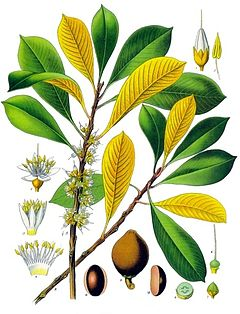
\includegraphics[width=0.50000\textwidth]{Sapotaceae.jpg}
\caption{hojas, flores y fruto de la familia Sapotaceae\label{imagen}}
\end{figure}

\begin{longtable}[]{@{}lllll@{}}
\toprule
p1 & p2 & p3 & p4 & p5\tabularnewline
\midrule
\endhead
10 & 16 & 62 & 33 & 34\tabularnewline
20 & 15 & 22 & 32 & 32\tabularnewline
30 & 38 & 23 & 12 & 46\tabularnewline
\bottomrule
\end{longtable}

\section{Metodología}\label{metodologuxeda}

\ldots

\section{Resultados}\label{resultados}

En toda la parcela, se registró un total de 2029 pertenecientes a 5
especies. La riqueza por cuadro fue de 4 especies y la mediana de la
abundancia por cuadro fue de 39 individuos. La especie más abundante fue
\emph{Pouteria reticulata}, con 1084 individuos, y la menos abundante
fue \emph{Pouteria fossicola} con 3 individuos. La tabla
\ref{tab:abun_sp} y la figura \ref{fig:abun_sp_q} resume estos
resultados.

\begin{longtable}[]{@{}lr@{}}
\caption{\label{tab:abun_sp}Abundancia por especie de la familia
Sapotaceae}\tabularnewline
\toprule
Latin & n\tabularnewline
\midrule
\endfirsthead
\toprule
Latin & n\tabularnewline
\midrule
\endhead
Pouteria reticulata & 1084\tabularnewline
Chrysophyllum argenteum & 711\tabularnewline
Chrysophyllum cainito & 171\tabularnewline
Pouteria stipitata & 60\tabularnewline
Pouteria fossicola & 3\tabularnewline
\bottomrule
\end{longtable}

\begin{figure}
\centering
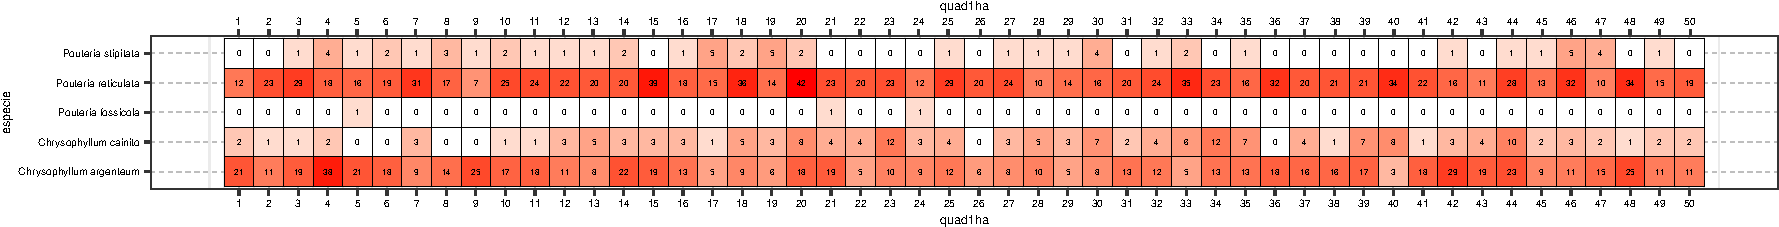
\includegraphics{manuscrito_files/figure-latex/unnamed-chunk-3-1.pdf}
\caption{\label{fig:abun_sp_q}Abundancia por especie por quadrat}
\end{figure}

\begin{figure}
\centering
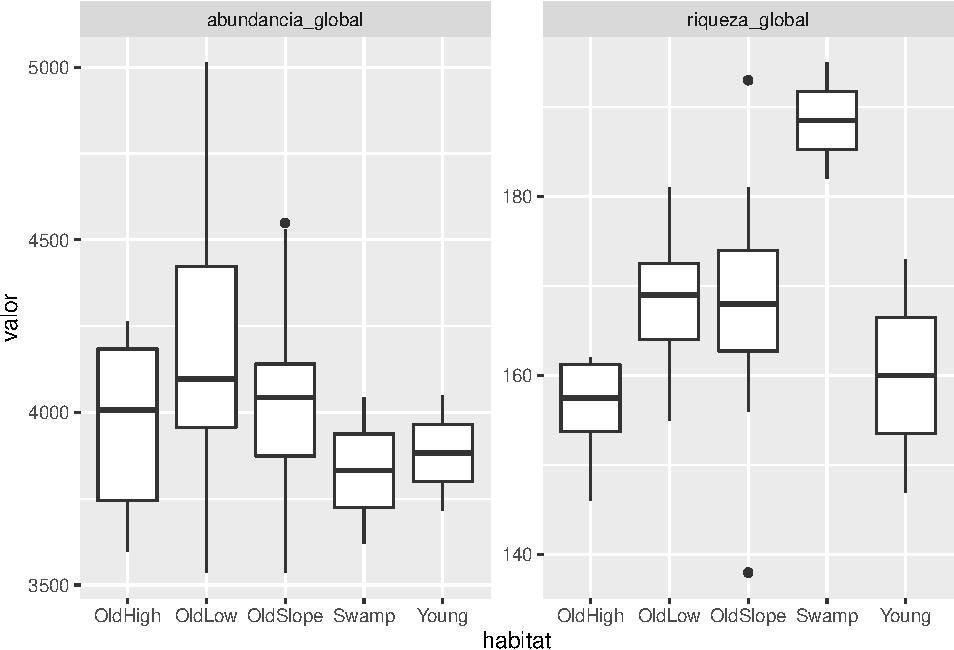
\includegraphics{manuscrito_files/figure-latex/unnamed-chunk-4-1.pdf}
\caption{\label{fig:P13}Diagrama de cajas de la abundancia y riqueza
segun habitats}
\end{figure}

la distribucion de la riqueza numerica de especies de la familia
Sapotaceae sigue un patron homogeneo, lo cual los agregados de riqueza
maxima estan distribuidos en casi todo el area. (ver Figura
\ref{fig:mapa_cuadros_riq_mi_familia})

\begin{figure}
\centering
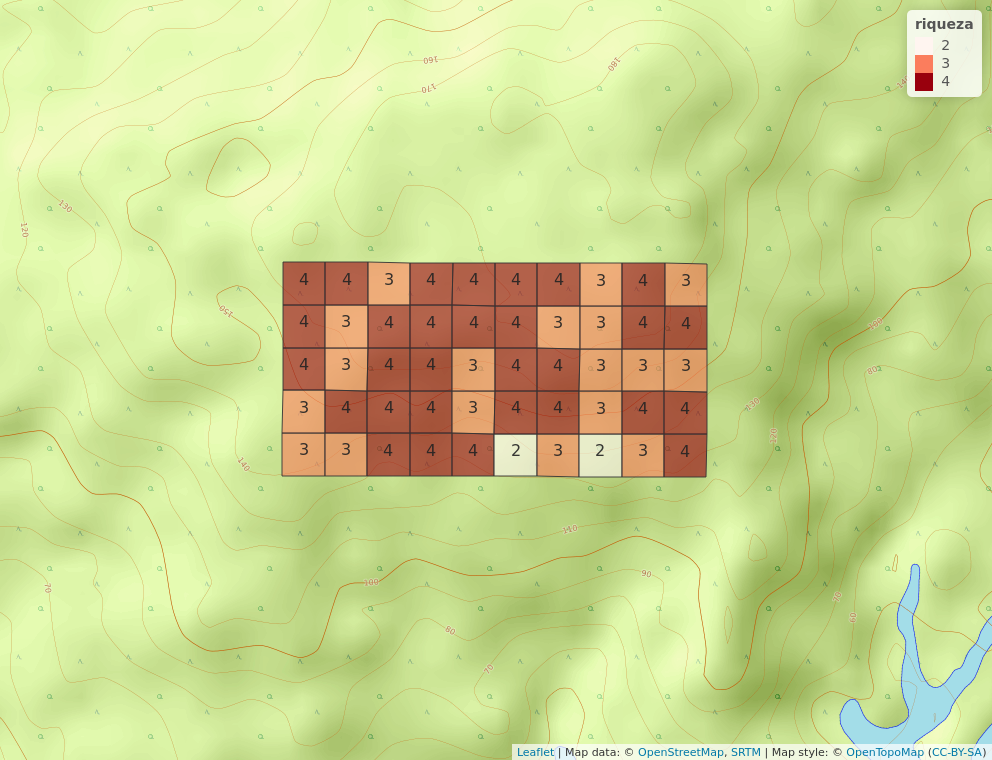
\includegraphics[width=0.50000\textwidth]{mapa_cuadros_riq_mi_familia.png}
\caption{Distribucion de la riqueza de la familia
Sapotaceae\label{fig:mapa_cuadros_riq_mi_familia}}
\end{figure}

Las variables ambientales pH y pendiente media presentaron asociacion
con la familia de plantas\ldots{}, lo cual supone\ldots{} (ver figuras
\ref{fig:mapa_cuadros_pH} y \ref{fig:mapa_cuadros_pendiente}).

\begin{figure}
\centering
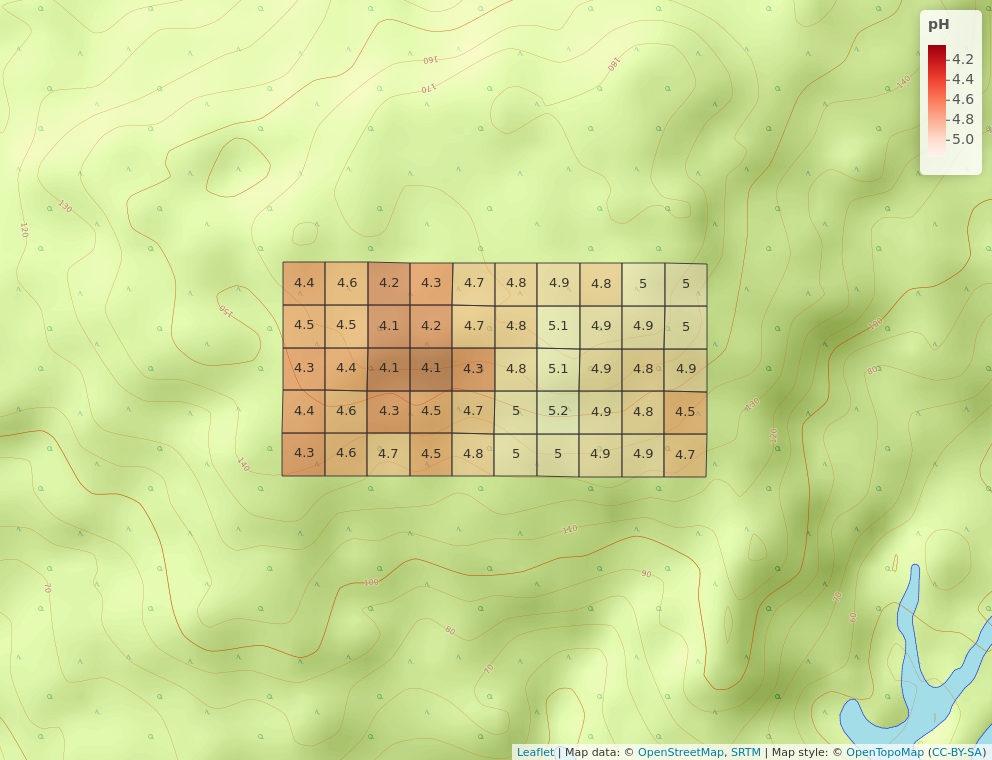
\includegraphics[width=0.50000\textwidth]{mapa_cuadros_ph.png}
\caption{Distribucion del pH\label{fig:mapa_cuadros_pH}}
\end{figure}

\begin{figure}
\centering
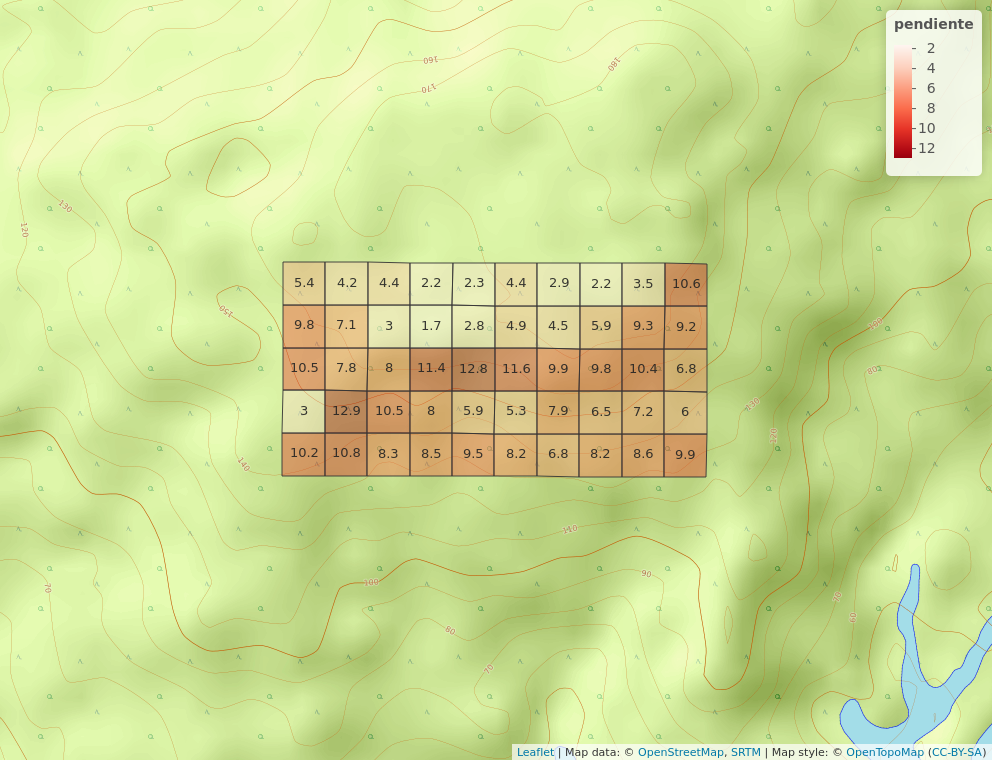
\includegraphics[width=0.50000\textwidth]{mapa_cuadros_pendiente.png}
\caption{Distribucion de las pendientes(en
grados)\label{fig:mapa_cuadros_pendiente}}
\end{figure}

la abundancia de la familia sapotaceae solo presenta correlacion con la
abundacia global, mientras que la riqueza tiene correlacion con la
presencia de cobre y nitrogeno en el suelo, lo que sugiere\ldots{} (ver
figura \ref{fig:p_cor_suelo_ar}).

\begin{figure}
\centering
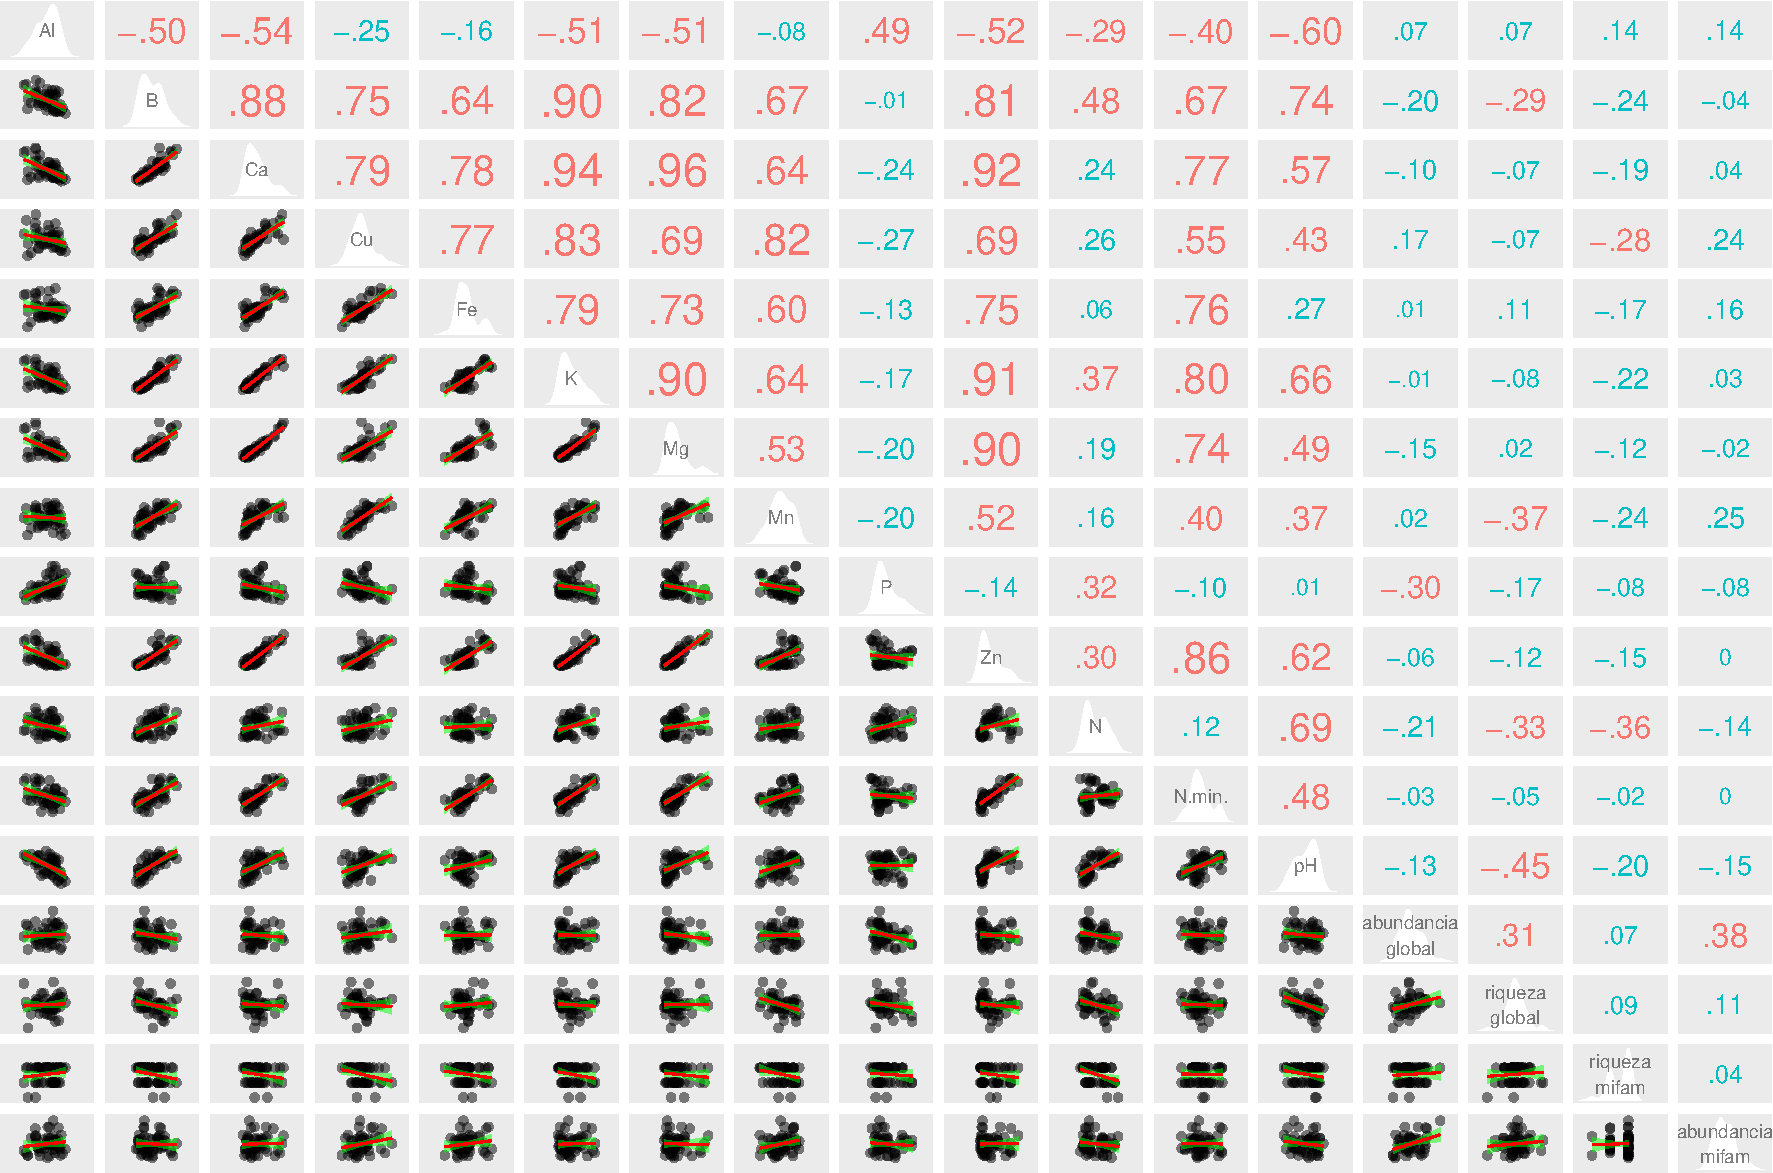
\includegraphics{manuscrito_files/figure-latex/unnamed-chunk-5-1.pdf}
\caption{\label{fig:p_cor_suelo_ar}correlacion de las variables del
suelo}
\end{figure}

las variables ambientales numericas y nominales presentan un patron (ver
figuras \ref{fig:mapas_variables_ambientales_numericas} y
\ref{fig:mapas_variables_ambientales_nominales}).

\begin{figure}
\centering
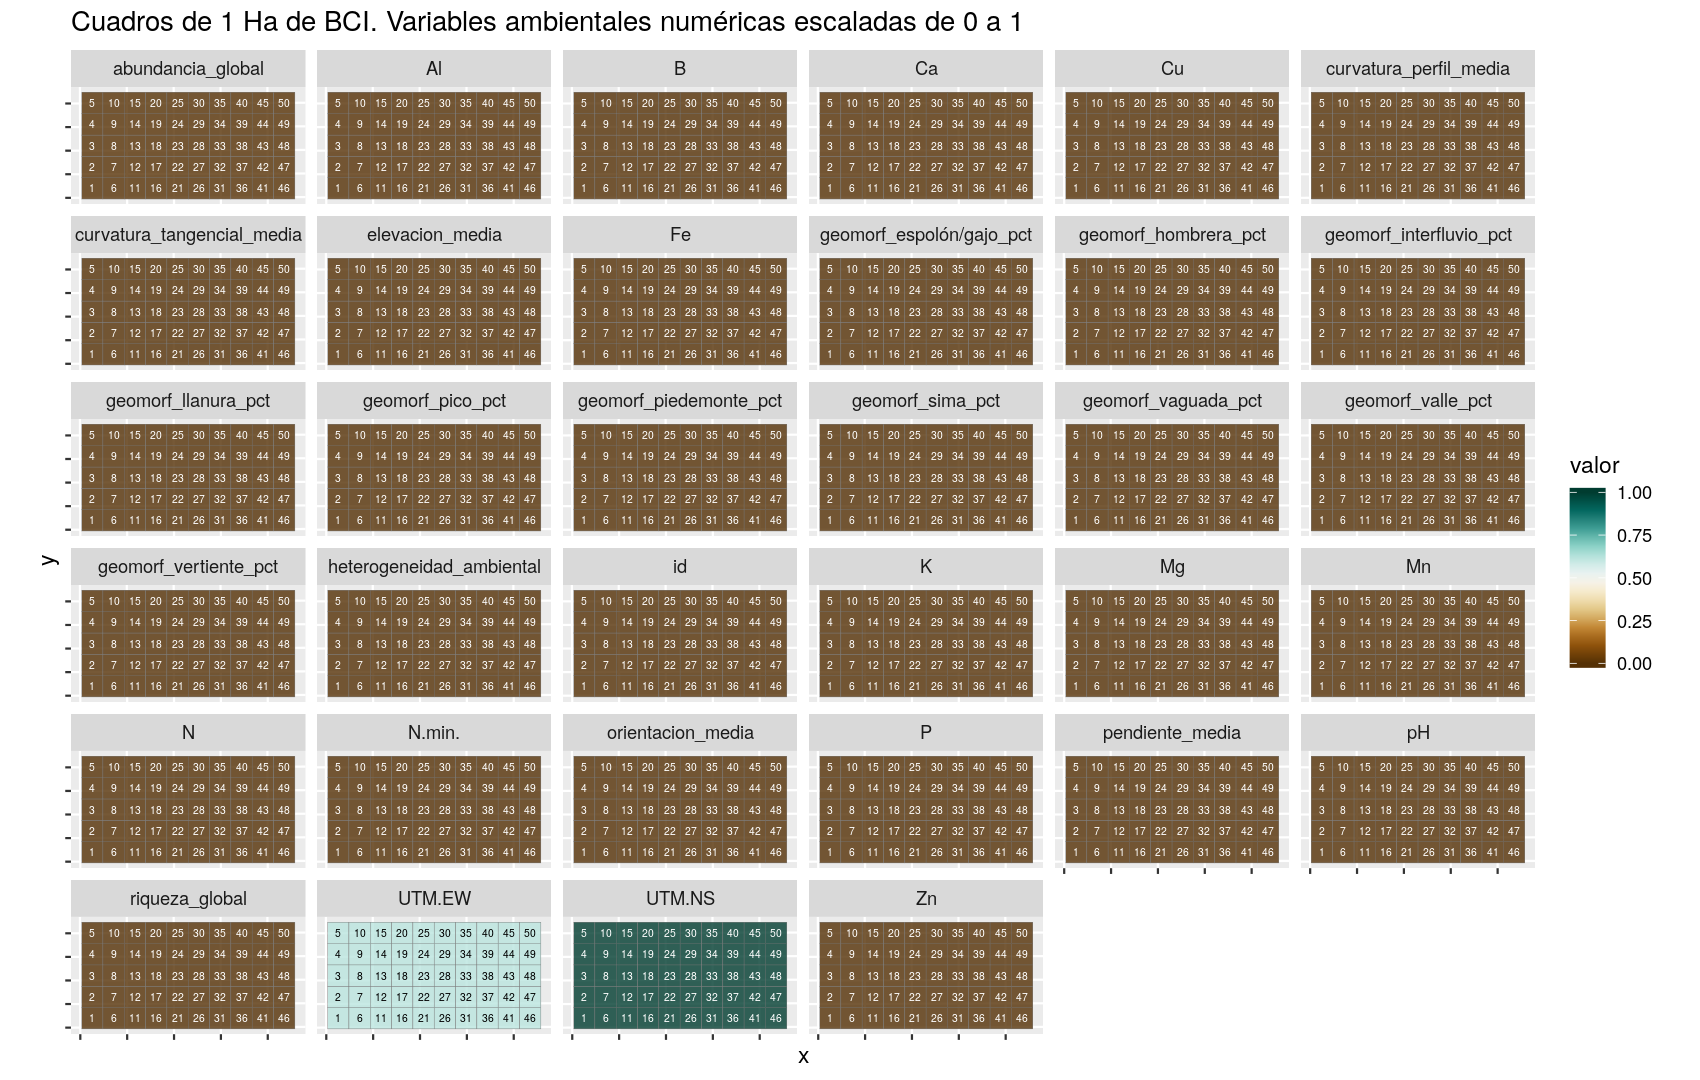
\includegraphics[width=1.00000\textwidth]{mapas_variables_ambientales_numericas.png}
\caption{variables ambientales
numericas\label{fig:mapas_variables_ambientales_numericas}}
\end{figure}

\begin{figure}
\centering
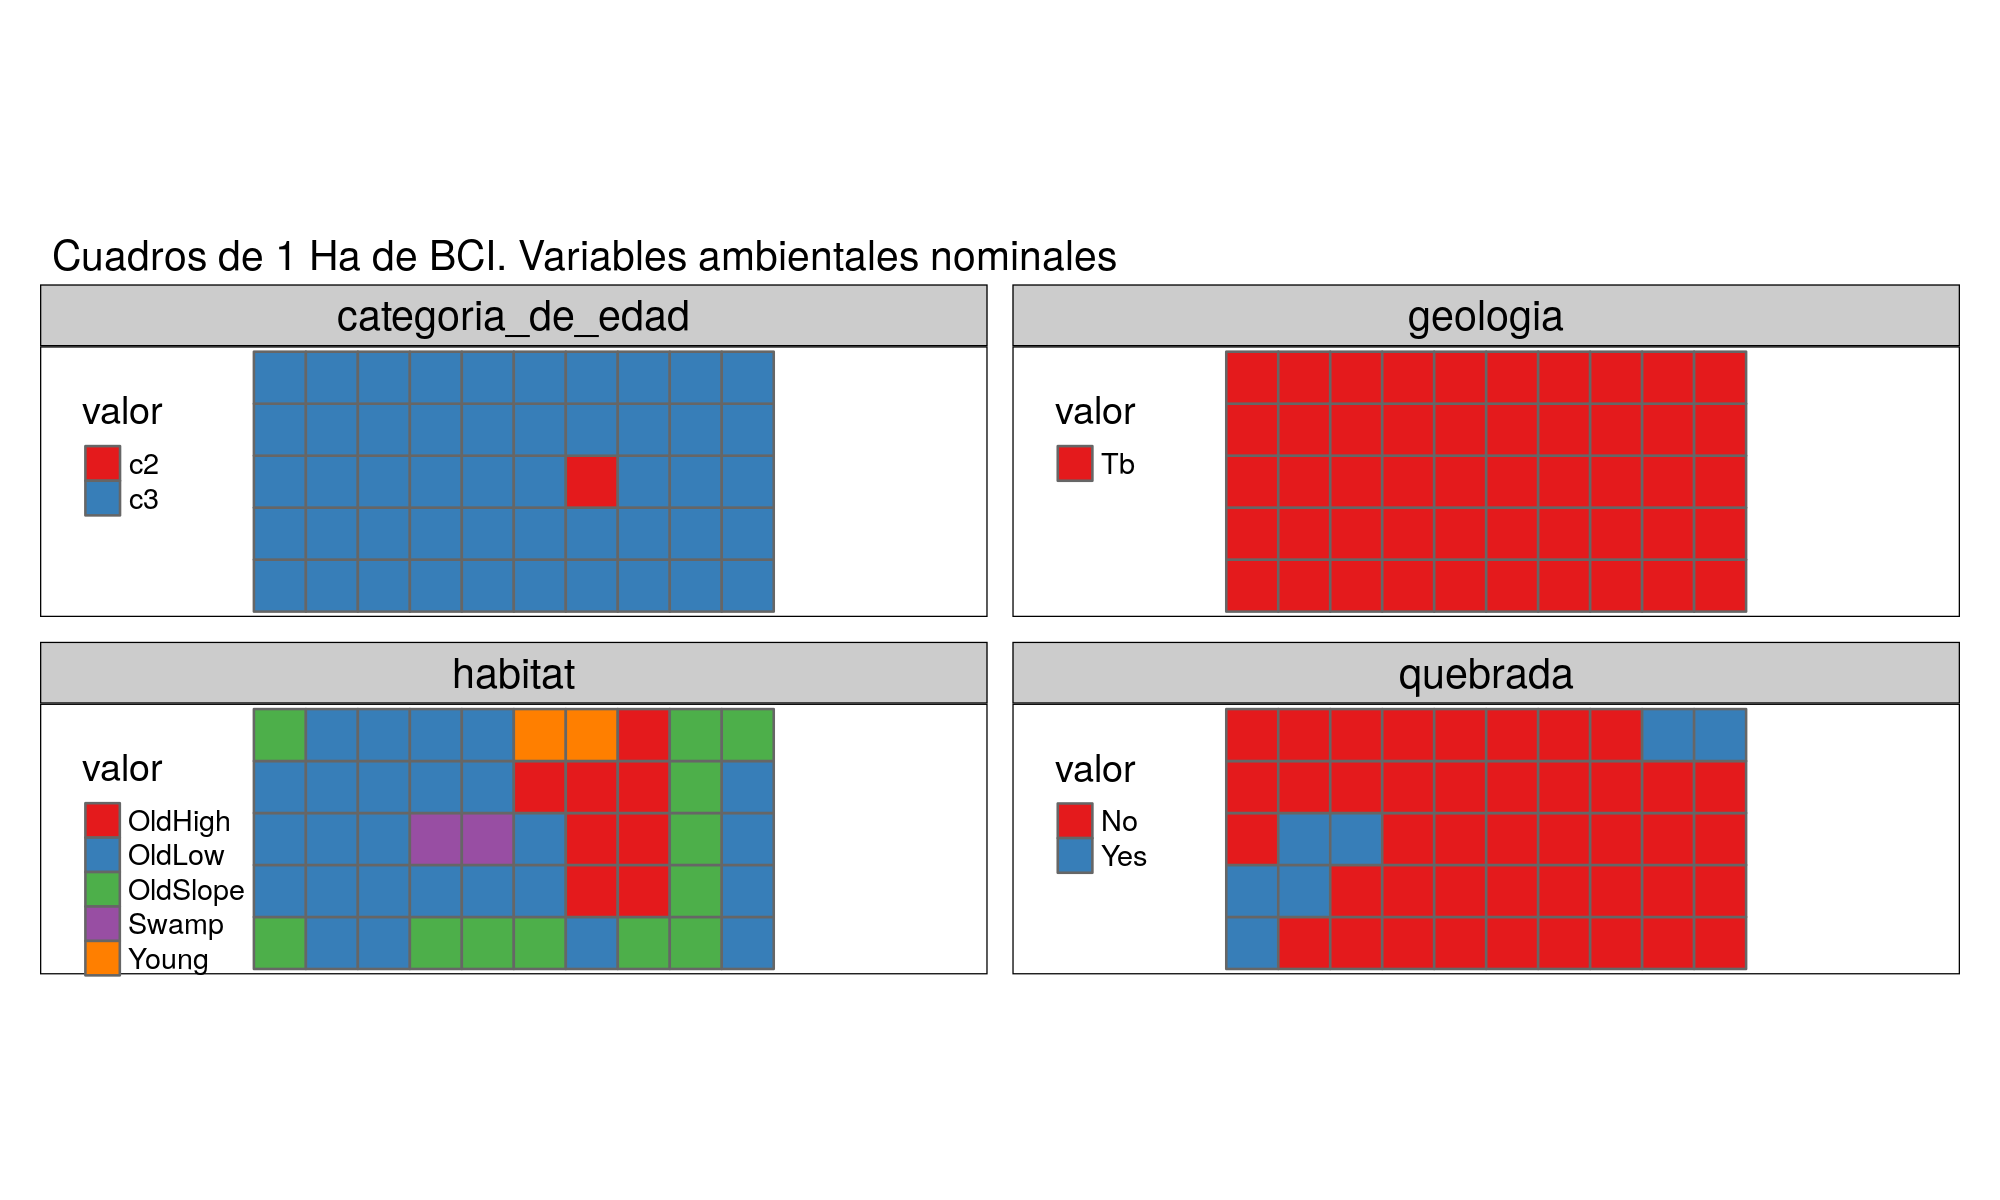
\includegraphics{mapas_variables_ambientales_nominales_tmap.png}
\caption{variables ambientales
nominales\label{fig:mapas_variables_ambientales_nominales}}
\end{figure}

El indice de similaridad de Jaccard muestra que el sitio 1 y 2 comparten
un 100\% de sus especies, por lo que ambos sitios comparten 3 especies y
no tienen especies exclusivas (ver figura
\ref{fig:similaridad_jaccard}).

\begin{figure}
\centering
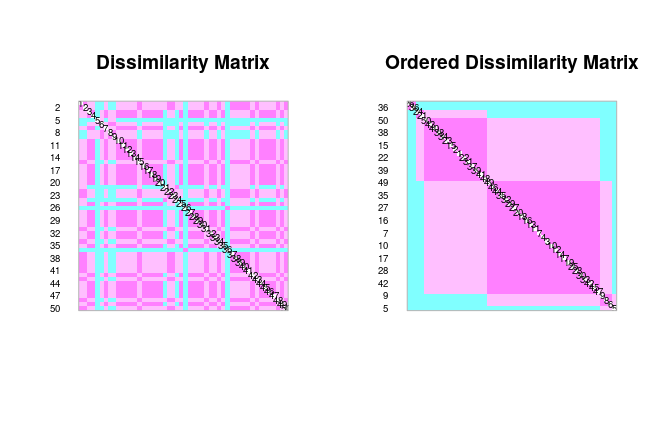
\includegraphics{medicion_asociacion_jaccard.png}
\caption{Similaridad de Jaccard(color fucsia (magenta, rosa) significa
``corta distancia=muy similares'', y cian (celeste) significa ``gran
distancia=poco similares'')\label{fig:similaridad_jaccard}}
\end{figure}

La correlcion entre las variables geomorfologicas con la abundancia y
riqueza\ldots{}(ver figura
\ref{fig:matriz_correlacion_geomorf_abun_riq_spearman}).

\begin{figure}
\centering
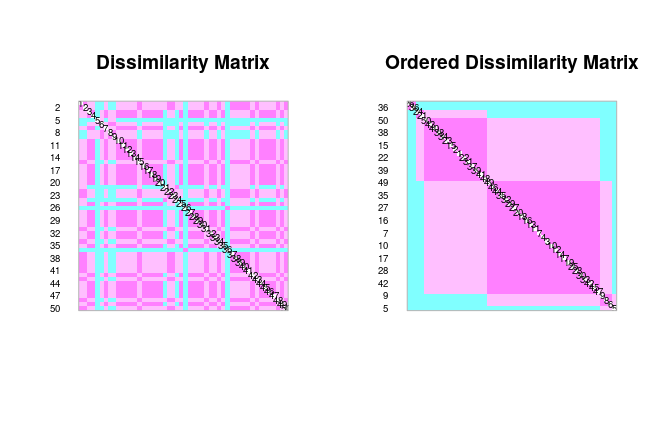
\includegraphics{medicion_asociacion_jaccard.png}
\caption{Panel de correlacion de Spearman entre los datos de la
comunidad y las variables
geomorfologicas\label{fig:matriz_correlacion_geomorf_abun_riq_spearman}}
\end{figure}

Las pruebas de correlación entre los grupos 1 y 2 formulados por
upgma\ldots{}(ver figura \ref{fig:{width=100%}}).

\begin{figure}
\centering
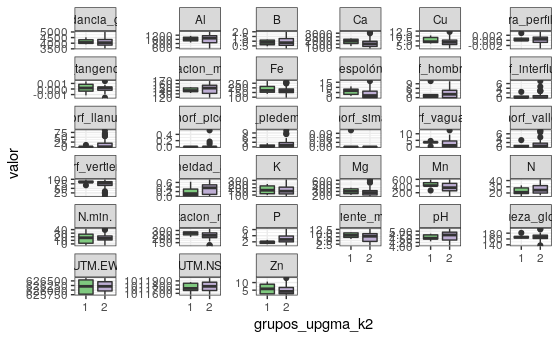
\includegraphics[width=1.00000\textwidth]{actualizacion_grupos_upgma.png}
\caption{Diagramas de caja de las variables que tuvieron un efecto,
segun las pruebas de igualdad de medias\label{fig:grupos_upgma}}
\end{figure}

La repartición de sitios en los grupos formulados por enlace
upgm\ldots{}(ver figura \ref{fig:mapa_upgma_k2}).

\begin{figure}
\centering
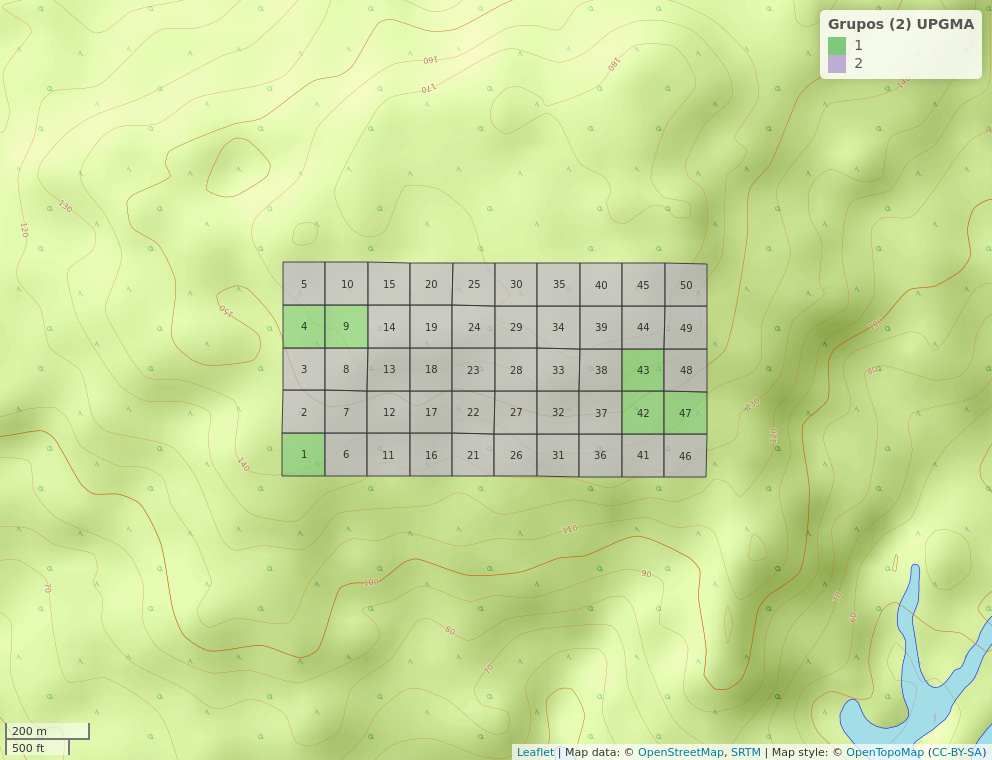
\includegraphics{mapa_upgma_k2.png}
\caption{Mapa en el que se presenta la distribucion de sitios en los
grupos formulados por enlace upgma\label{fig:mapa_upgma_k2}}
\end{figure}

Las especies indicadoras fueron\ldots{}(verificar analisis de
agrupamiento 4)

Análisis de especies indicadoras mediante IndVal Association function:
IndVal.g Significance level (alpha): 0.05

Total number of species: 5 Selected number of species: 2 Number of
species associated to 1 group: 2

List of species associated to each combination:

Group 1 \#sps. 1 A B stat p.value\\
Chrysophyllum argenteum 0.6565 1.0000 0.81 0.005 **

Group 2 \#sps. 1 A B stat p.value\\
Pouteria reticulata 0.6505 1.0000 0.807 0.001 ***

grado de correlacion que existe en cado uno de los indices\ldots{} (ver
figura \ref{fig:correlacion_indices}).

\begin{figure}
\centering
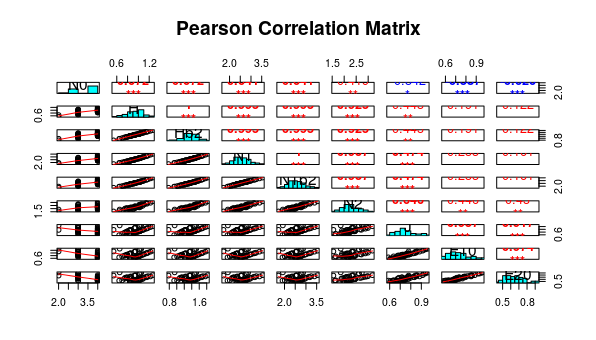
\includegraphics[width=1.00000\textwidth]{correlacion_indices.png}
\caption{Grado de correlacion entre cado uno de los indices. N0: riqueza
de especies; H: entropia de Shannon; Hb2: entropia de Shannon con 2 como
base del logaritmo; N1 y N2: Numeros de Hill; N1b2: Numero de Hill 1 en
base log 2; J: equidad de Pielou; E10 y E20: ratios de Hill 1 y 2
\label{fig:correlacion_indices}}
\end{figure}

La riqueza de la familia Sapotaceae aumenta en función del contenido de
hierro, nitrógeno y cobre, tambien aunmenta con la equidad (ver figura
\ref{fig:correlacion_diversidad_equidad}).

\begin{figure}
\centering
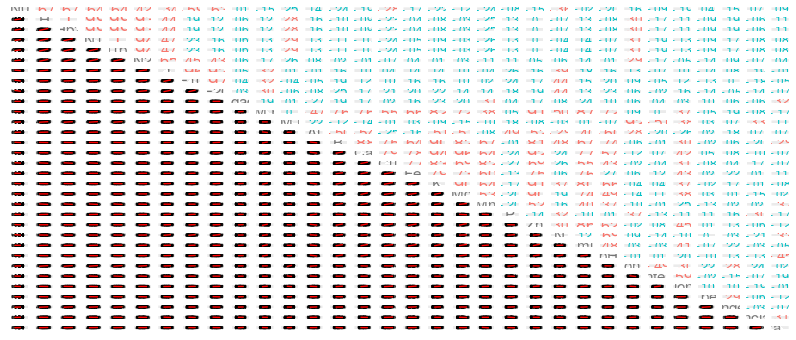
\includegraphics[width=0.50000\textwidth]{correlacion_diversidad_equidad.png}
\caption{Correlacion entre diversidad/equidad y algunas de las variables
ambientales \label{fig:correlacion_diversidad_equidad}}
\end{figure}

Sitios que tienen mayores valores de equidad (azul y verde)\ldots{} (ver
figura \ref{fig:grafico_niveles_equidad}).

\begin{figure}
\centering
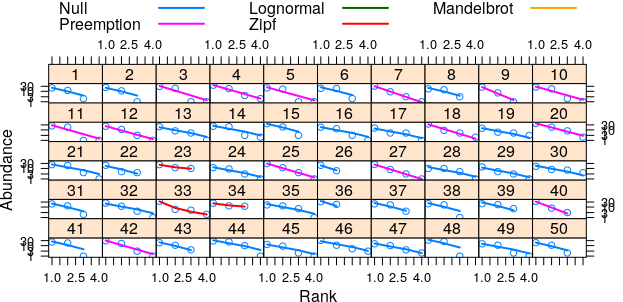
\includegraphics{grafico_niveles_equidad.png}
\caption{Grafico dque presenta los valores de equidad por sitos
\label{fig:grafico_niveles_equidad}}
\end{figure}

Curva de rarefaccion de los sitios, teniendo en cuenta la riqueza y la
abundancia\ldots{}(ver figura \ref{fig:Curva_rarefaccion}). analizar
Analisis de diversidad 1

\begin{figure}
\centering
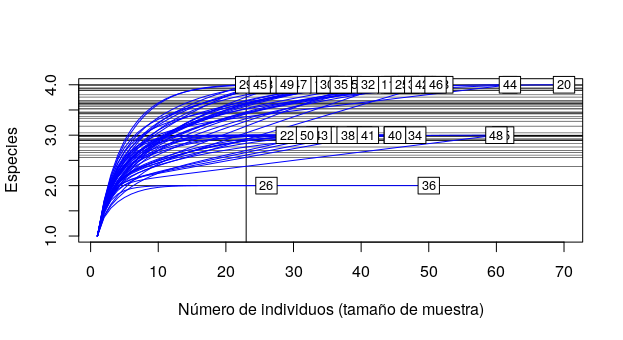
\includegraphics{Curva_rarefaccion.png}
\caption{Curva de rarefaccion de los sitios
\label{fig:Curva_rarefaccion}}
\end{figure}

asymptotic diversity estimates along with related statistics. Observed
Estimator Est\_s.e. 95\% Lower 95\% Upper Species Richness 5.000 5.000
0.217 5.000 5.481 Shannon diversity 2.786 2.789 0.045 2.786 2.876
Simpson diversity 2.403 2.404 0.038 2.403 2.478

Acumulacion de especies en funcion de numeros de individuos\ldots{}(ver
figura \ref{fig:acumulacion_especies_individuos}).

\begin{figure}
\centering
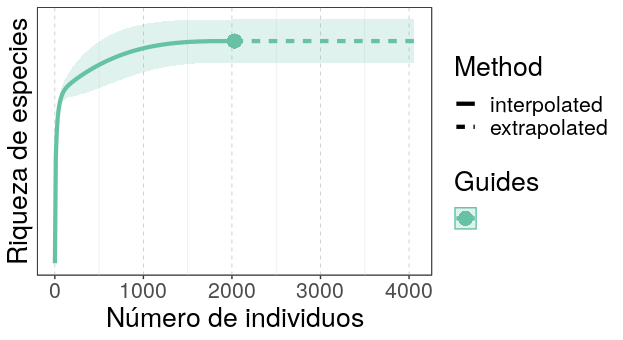
\includegraphics{acumulacion_especies_individuos.png}
\caption{Grafico de acumulacion de especies en funcion de numeros de
individuos \label{fig:acumulacion_especies_individuos}}
\end{figure}

Valores de diversidad beta por cada una de las especies y cuales son su
contribucion (comparar cueles son las especies que contribuyen mas a la
diveridad beta) especies\_contribuyen\_betadiv Chrysophyllum argenteum
Chrysophyllum cainito Pouteria stipitata 0.2504234 0.3147978 0.2658814

\$sitios\_contribuyen\_betadiv {[}1{]} ``9'' ``40''

Estos sitios presentan contribucion a la diversidad beta por la
incidencia de algunas variables ambientales (habitat, y variables
numericas\ldots{})(ver figura
\ref{fig:mapas_variables_ambientales_numericas} y
\ref{fig: mapas_variables_ambientales_nominales}).

Componentes príncipales de la varianza en las variables de suelo y
geomorfología en BCI.En estos gráficos se incluye el comportamiento de
la varianza explicada, predecido por el modelo de bara quebrada,
representado por la línea roja formando la curva. (La escala denominada
``Inertia'' representa la suma de los cuadrados de toda la varianza)
(ver figura \ref{fig:env_suelo_pca}).

\begin{figure}
\centering
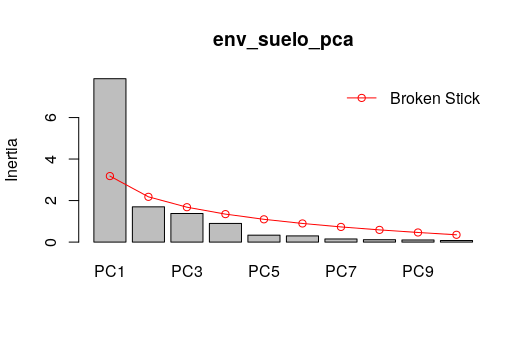
\includegraphics{env_suelo_pca.png}
\caption{grafico de los componentes principales de la varianza en las
variables suelo y geomorfologia en BCI \label{fig:env_suelo_pca}}
\end{figure}

Se observa que las variables nitrógeno, fósforo y pH aportan la mayor
parte de la varianza explicada. La relación entre las variables se
encuentra debidamente representada en el recuadro del escalamiento 2,
por medio delos ángulos que forman sus vectores (ver figura
\ref{fig:Biplot_PCA_escalamiento}).

\begin{figure}
\centering
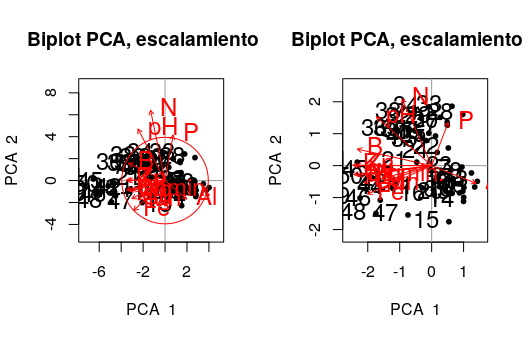
\includegraphics[width=1.00000\textwidth]{Biplot_PCA_escalamiento.png}
\caption{Biplots generados en el PCA de las viariables de suelo
\label{fig:Biplot_PCA_escalamiento}}
\end{figure}

El escalamiento 1, muestra muchos de los cuadrantes dispuestos alrededor
del origen formado por los ejes, lo que indica una contribución a la
varianza relativamente equitativa por parte de las especies. Sin
embargo, aparecen también unos cuantos cuadrantes con valores atípicos y
más alejados. Se nota como las especies (mencionar especies) presentan
una contribución desproporcionada a la varianza total, en comparación
con el resto de las especies (ver figura \ref{fig:PCA_comunidad}).

\begin{figure}
\centering
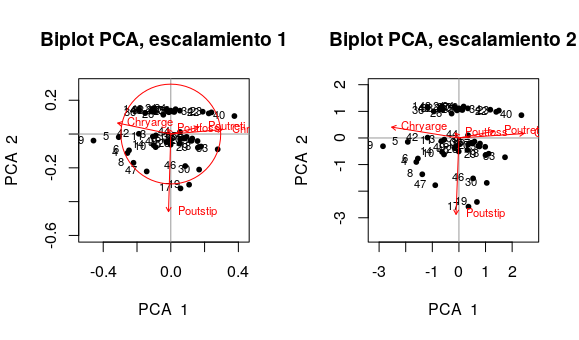
\includegraphics[width=1.00000\textwidth]{PCA_comunidad.png}
\caption{Biplots generados en el PCA de las viariables de suelo
\label{fig:PCA_comunidad}}
\end{figure}

Biplot del análisis de correspondencia de los datos de abundancia de las
especies de Sapotaceae (ver figura
\ref{fig:Analisis_de_correspondencia}).

\begin{figure}
\centering
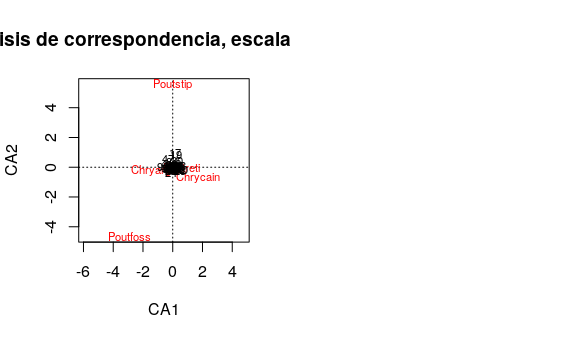
\includegraphics[width=1.00000\textwidth]{Analisis_de_correspondencia.png}
\caption{Biplot del analisis de correspondencia de los datos de
abundancia de las especies de Sapotaceae
\label{fig:Analisis_de_correspondencia}}
\end{figure}

(ver figura \ref{fig:PCoA _promedios_especies}).

\begin{figure}
\centering
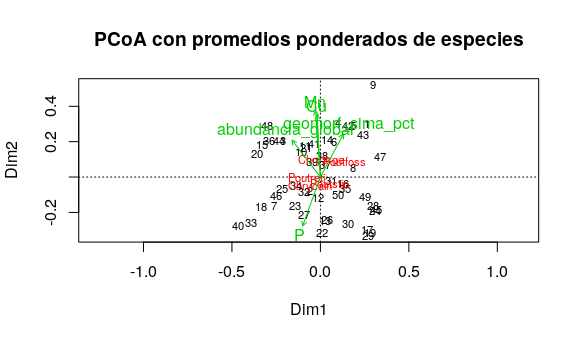
\includegraphics[width=1.00000\textwidth]{PCoA _promedios_especies.png}
\caption{PCoA con promedios ponderados de especies
\label{fig:PCoA _promedios_especies}}
\end{figure}

\section{Discusión}\label{discusiuxf3n}

\section{Agradecimientos}\label{agradecimientos}

\section{Información de soporte}\label{informaciuxf3n-de-soporte}

\ldots

\section{\texorpdfstring{\emph{Script}
reproducible}{Script reproducible}}\label{script-reproducible}

\ldots

\section*{Referencias}\label{referencias}
\addcontentsline{toc}{section}{Referencias}

\hypertarget{refs}{}
\hypertarget{ref-henriquez2012fenologia}{}
Henríquez, C. A., Sotes, G. J., \& Bustamante, R. O. (2012). Fenología
reproductiva de pouteria splendens (sapotaceae). \emph{Gayana.
Botánica}, \emph{69}(2), 251--255.

\hypertarget{ref-martinez2020importancia}{}
Martínez-Sovero, G., Iglesias-Osores, S., \& Villena-Velásquez, J. J.
(2020). Importancia de la familia sapotaceae en madre de dios, perú.
\emph{Manglar}, \emph{17}(4), 287.




\newpage
\singlespacing 
\end{document}
